\subsection{HOG-SVM}  
For our HOG-SVM feature type / classifier combination we used locally normalized histogram of oriented gradients (HOG) descriptors \cite{citeulike:335784} as the feature type and a multiclass model for support vector machine as the classifier. The method takes an input image which is normalized for gamma and colour for better invariance to factors such as illumination and shadowing, then a grid is placed on the image and for every cell a histogram of oriented gradient features is extracted, the concept being local object appearance and shape are characterized by a distribution of intensity gradients or edge positions. Each cell holds a 1-D histogram of gradients and edge orientations over the pixel of the cell, noting that the referenced work applied to human detection in general. 

We defined function \textbf{fnCreateHOGSVMClassifier} to create a multiclass model for support vector machine using matlab function \textbf{fitcecoc}, and script \textbf{TrainNetworks.m} to test different classifiers, using code supplied in lab 6 \cite{INM460-lab-wk6} with some modifications. Data was split at a ratio of 90\%/10\% for training and testing. Training data was then run through the feature extraction function  \textbf{extractHOGFeatures}, which generated our encoded shape information. Since we had to somehow turn the features into a vector to be used by our Support Vector Machine classifier, we chose to use grayscale images as the intuition was this approach would constrain the task and make it more manageable - see section \ref{Discussion-marker}. We tested different cell sizes; [50 50], [25 25] and [10 10], finding that smaller cell sizes generated a larger number of HOG features, as well as higher accuracies. The data generated from our grid search is shown in Table \ref{table:hog_stats}, section \ref{Appendix}. Given the feature length was not necessarily the same for each image and smaller cell sizes generated more features, we defined a value of 2500 features, which in most cases exceeded the number of features extracted for each image. We then used this value to adjust the size of the vector that would be used to train our SVM. If the feature vector returned by \textbf{extractHOGFeatures} was greater, we shortened the vector, and if it was less, we padded the feature vector with zeros, to ensure the final feature vector was always equal to our defined feature size.

The same process, as implemented in function \textbf{fnHOGSMVPredict}, was used when classifying unseen group images. HOG features were extracted, vector size adjusted before being passed to the SMV classifier.

Our best HOG-SVM model accuracy was 0.9990 (Table \ref{table:acc_table}). Since we had a total of 48 labels, the resulting confusion matrix was not readable, so we created a subset with 8 labels with the same 200 images for each label, generating the confusion matrix shown in Figure \ref{fig:hog_conf_mat} with approximately the same accuracy. 

\begin{figure}[h]
 \centering 
 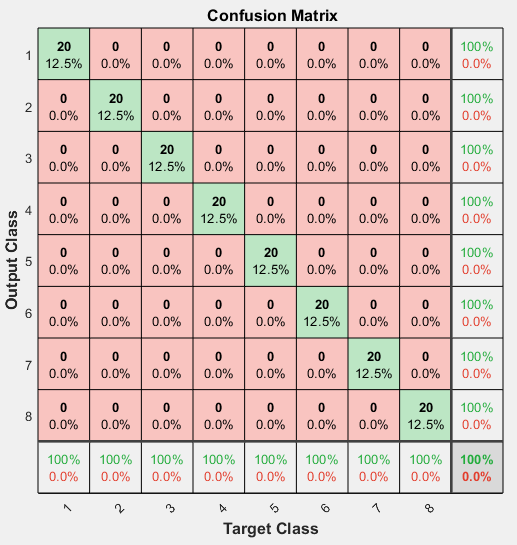
\includegraphics[width=\columnwidth]{images/HOG-SVM-Conf-Mat-200-gray-0.9.png}
 \caption{HOG SVM Confusion Matrix, 8 labels, 200 images each, 90\%/10\% train/test split}
 \label{fig:hog_conf_mat}
\end{figure}  
The widely different accuracy obtained from testing individual labelled images and testing group images (Tables \ref{table:acc_table} and \ref{table:acc_table_group}) suggests the model is overfitting. We discuss this in section \ref{Discussion-marker}.


